\documentclass{standalone}
\usepackage{tikz}
\usetikzlibrary{patterns, positioning}
\usepackage[sfdefault]{ClearSans} %% option 'sfdefault' activates Clear Sans as the default text font
\usepackage[T1]{fontenc}

\begin{document}
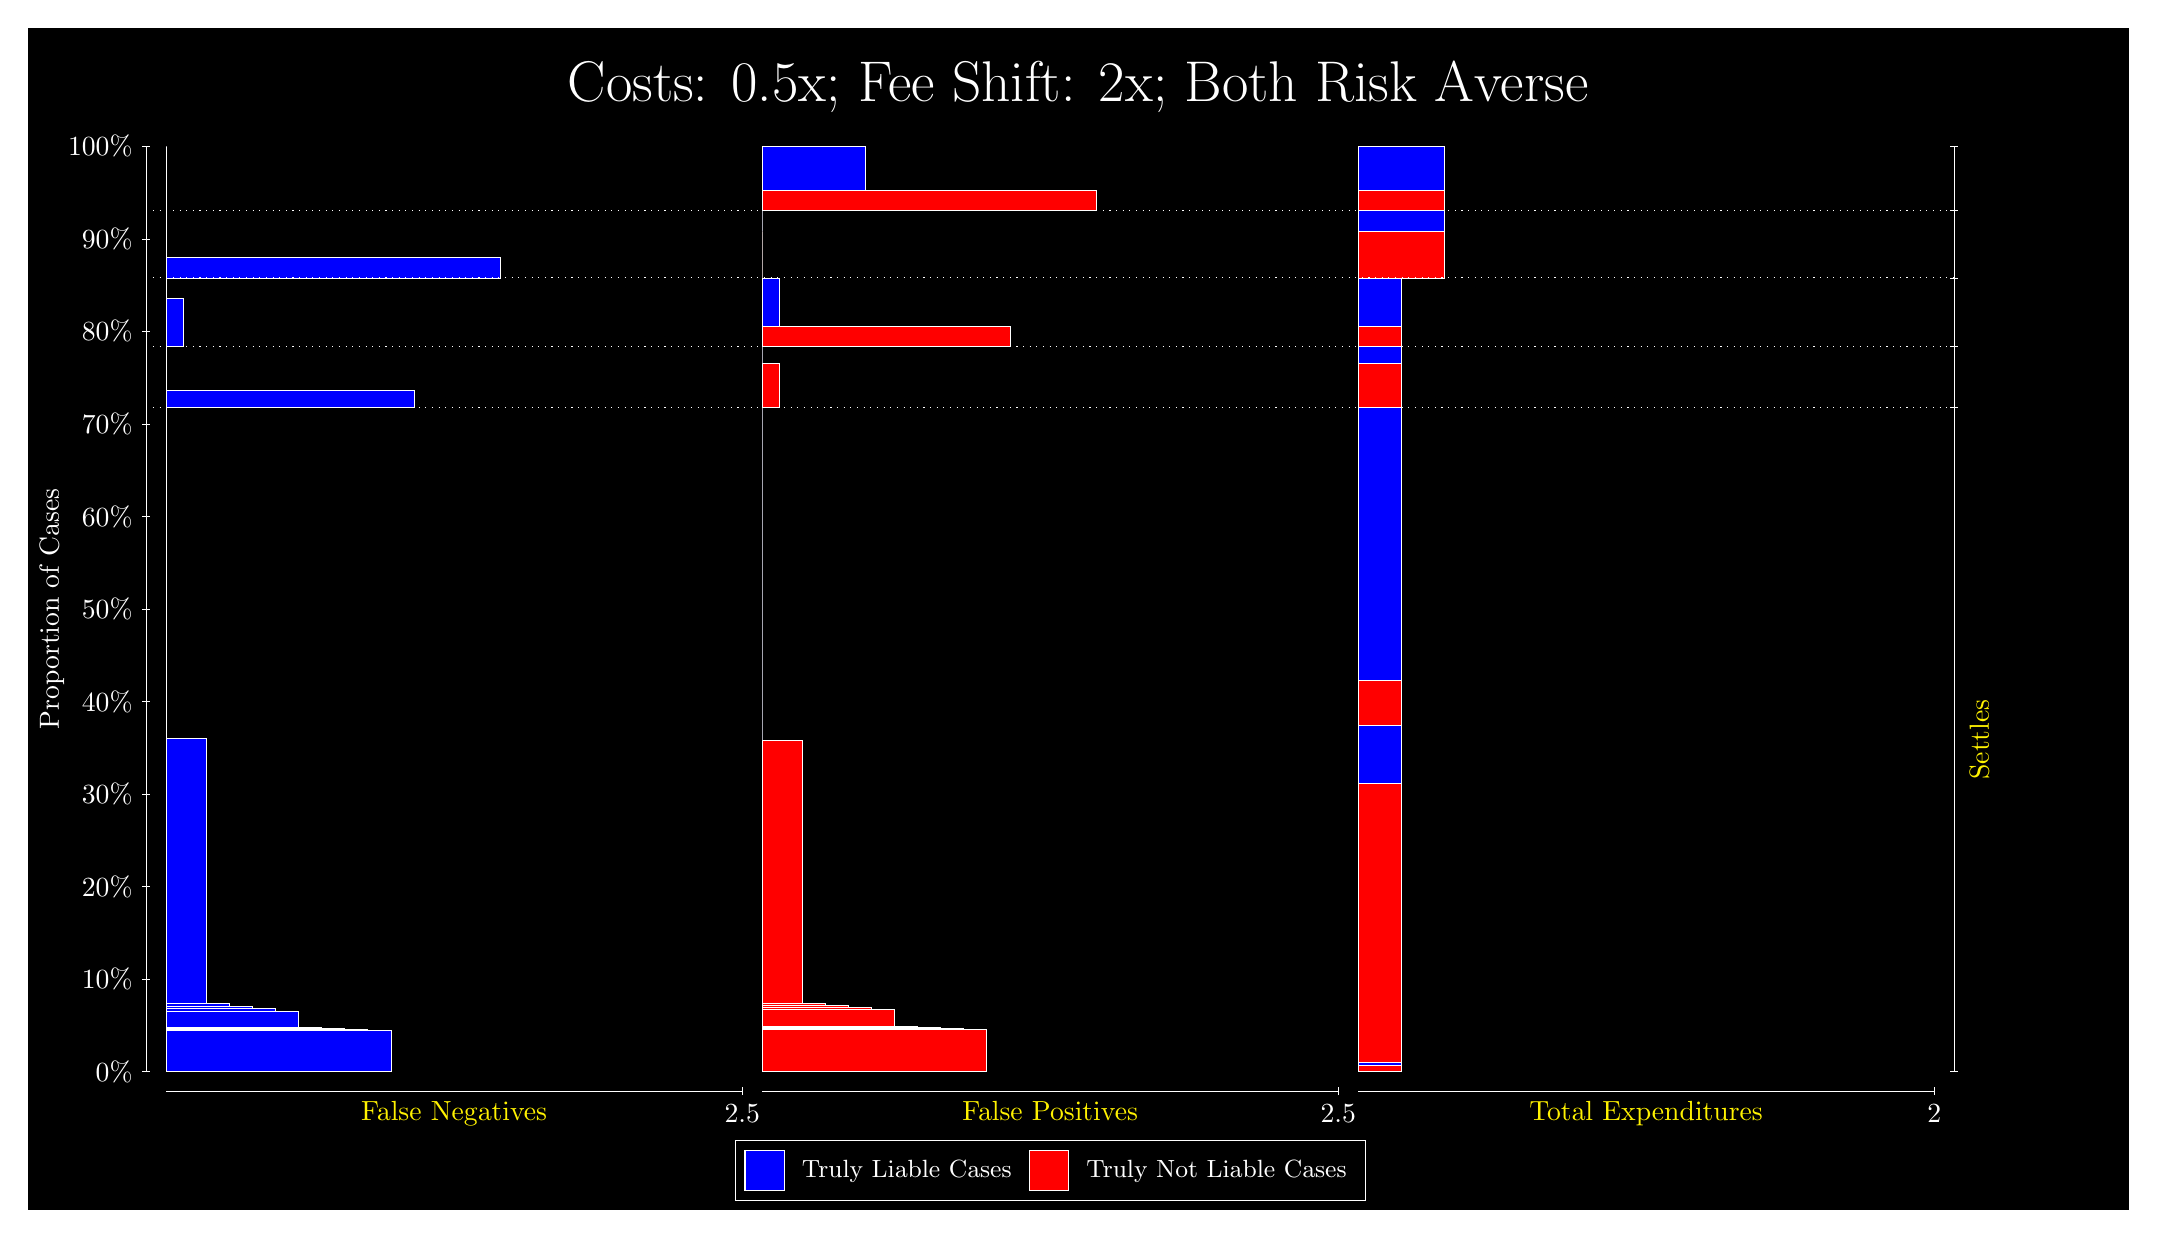
\begin{tikzpicture}
\draw[fill=black] (0,0) rectangle (26.667,15);
\draw[text=white] (0,13.5) rectangle (26.667,15) node[midway] {\huge Costs: 0.5x; Fee Shift: 2x; Both Risk Averse};
\draw[white, very thin] (1.5,1.75) -- (1.5,13.5);
\node[rotate=90, text=white, anchor=center] at (0.3, 7.625) {Proportion of Cases};
\draw[white, very thin] (1.45,1.75) -- (1.55,1.75);
\node[text=white, anchor=east] at (1.45, 1.75) {0\%};
\draw[white, very thin] (1.45,2.925) -- (1.55,2.925);
\node[text=white, anchor=east] at (1.45, 2.925) {10\%};
\draw[white, very thin] (1.45,4.1) -- (1.55,4.1);
\node[text=white, anchor=east] at (1.45, 4.1) {20\%};
\draw[white, very thin] (1.45,5.275) -- (1.55,5.275);
\node[text=white, anchor=east] at (1.45, 5.275) {30\%};
\draw[white, very thin] (1.45,6.45) -- (1.55,6.45);
\node[text=white, anchor=east] at (1.45, 6.45) {40\%};
\draw[white, very thin] (1.45,7.625) -- (1.55,7.625);
\node[text=white, anchor=east] at (1.45, 7.625) {50\%};
\draw[white, very thin] (1.45,8.8) -- (1.55,8.8);
\node[text=white, anchor=east] at (1.45, 8.8) {60\%};
\draw[white, very thin] (1.45,9.975) -- (1.55,9.975);
\node[text=white, anchor=east] at (1.45, 9.975) {70\%};
\draw[white, very thin] (1.45,11.15) -- (1.55,11.15);
\node[text=white, anchor=east] at (1.45, 11.15) {80\%};
\draw[white, very thin] (1.45,12.325) -- (1.55,12.325);
\node[text=white, anchor=east] at (1.45, 12.325) {90\%};
\draw[white, very thin] (1.45,13.5) -- (1.55,13.5);
\node[text=white, anchor=east] at (1.45, 13.5) {100\%};

\draw[white, very thin] (24.457,1.75) -- (24.457,13.5);
\draw[white, very thin] (24.407,1.75) -- (24.507,1.75);
\node[anchor=west] at (24.407, 1.75) {};
\draw[white, very thin] (24.407,10.186) -- (24.507,10.186);
\node[anchor=west] at (24.407, 10.186) {};
\draw[white, very thin] (24.407,10.96) -- (24.507,10.96);
\node[anchor=west] at (24.407, 10.96) {};
\draw[white, very thin] (24.407,11.829) -- (24.507,11.829);
\node[anchor=west] at (24.407, 11.829) {};
\draw[white, very thin] (24.407,12.684) -- (24.507,12.684);
\node[anchor=west] at (24.407, 12.684) {};
\draw[white, very thin] (24.407,13.5) -- (24.507,13.5);
\node[anchor=west] at (24.407, 13.5) {};

\draw[white, very thin, fill=blue] (1.75,1.75) rectangle (4.6044,2.2754);
\draw[white, very thin, fill=blue] (1.75,2.2754) rectangle (4.3116,2.2853);
\draw[white, very thin, fill=blue] (1.75,2.2853) rectangle (4.0188,2.2968);
\draw[white, very thin, fill=blue] (1.75,2.2968) rectangle (3.7261,2.3093);
\draw[white, very thin, fill=blue] (1.75,2.3093) rectangle (3.4333,2.5202);
\draw[white, very thin, fill=blue] (1.75,2.5202) rectangle (3.1406,2.5509);
\draw[white, very thin, fill=blue] (1.75,2.5509) rectangle (2.8478,2.582);
\draw[white, very thin, fill=blue] (1.75,2.582) rectangle (2.5551,2.6124);
\draw[white, very thin, fill=blue] (1.75,2.6124) rectangle (2.2623,5.9834);
\draw[white, very thin, fill=red] (1.75,5.9834) rectangle (1.75,10.186);
\draw[white, very thin, fill=blue] (1.75,10.186) rectangle (4.8971,10.401);
\draw[white, very thin, fill=red] (1.75,10.401) rectangle (1.75,10.96);
\draw[white, very thin, fill=blue] (1.75,10.96) rectangle (1.9696,11.57);
\draw[white, very thin, fill=red] (1.75,11.57) rectangle (1.75,11.829);
\draw[white, very thin, fill=blue] (1.75,11.829) rectangle (5.9949,12.093);
\draw[white, very thin, fill=red] (1.75,12.093) rectangle (1.75,12.684);
\draw[white, very thin, fill=red] (1.75,12.684) rectangle (1.75,12.948);
\draw[white, very thin, fill=blue] (1.75,12.948) rectangle (1.75,13.5);
\draw[white, very thin, fill=red] (9.3189,1.75) rectangle (12.173,2.2855);
\draw[white, very thin, fill=red] (9.3189,2.2855) rectangle (11.88,2.2983);
\draw[white, very thin, fill=red] (9.3189,2.2983) rectangle (11.588,2.3119);
\draw[white, very thin, fill=red] (9.3189,2.3119) rectangle (11.295,2.3252);
\draw[white, very thin, fill=red] (9.3189,2.3252) rectangle (11.002,2.5384);
\draw[white, very thin, fill=red] (9.3189,2.5384) rectangle (10.709,2.5393);
\draw[white, very thin, fill=red] (9.3189,2.5393) rectangle (10.709,2.5681);
\draw[white, very thin, fill=red] (9.3189,2.5681) rectangle (10.417,2.5951);
\draw[white, very thin, fill=red] (9.3189,2.5951) rectangle (10.124,2.6192);
\draw[white, very thin, fill=red] (9.3189,2.6192) rectangle (9.8312,5.9522);
\draw[white, very thin, fill=blue] (9.3189,5.9522) rectangle (9.3189,10.186);
\draw[white, very thin, fill=red] (9.3189,10.186) rectangle (9.5384,10.745);
\draw[white, very thin, fill=blue] (9.3189,10.745) rectangle (9.3189,10.96);
\draw[white, very thin, fill=red] (9.3189,10.96) rectangle (12.466,11.219);
\draw[white, very thin, fill=blue] (9.3189,11.219) rectangle (9.5384,11.829);
\draw[white, very thin, fill=red] (9.3189,11.829) rectangle (9.3189,12.42);
\draw[white, very thin, fill=blue] (9.3189,12.42) rectangle (9.3189,12.684);
\draw[white, very thin, fill=red] (9.3189,12.684) rectangle (13.564,12.948);
\draw[white, very thin, fill=blue] (9.3189,12.948) rectangle (10.636,13.5);
\draw[white, very thin, fill=red] (16.888,1.75) rectangle (17.437,1.8308);
\draw[white, very thin, fill=blue] (16.888,1.8308) rectangle (17.437,1.8647);
\draw[white, very thin, fill=red] (16.888,1.8647) rectangle (17.437,5.4109);
\draw[white, very thin, fill=blue] (16.888,5.4109) rectangle (17.437,6.1472);
\draw[white, very thin, fill=red] (16.888,6.1472) rectangle (17.437,6.7224);
\draw[white, very thin, fill=blue] (16.888,6.7224) rectangle (17.437,10.186);
\draw[white, very thin, fill=red] (16.888,10.186) rectangle (17.437,10.745);
\draw[white, very thin, fill=blue] (16.888,10.745) rectangle (17.437,10.96);
\draw[white, very thin, fill=red] (16.888,10.96) rectangle (17.437,11.219);
\draw[white, very thin, fill=blue] (16.888,11.219) rectangle (17.437,11.829);
\draw[white, very thin, fill=red] (16.888,11.829) rectangle (17.986,12.42);
\draw[white, very thin, fill=blue] (16.888,12.42) rectangle (17.986,12.684);
\draw[white, very thin, fill=red] (16.888,12.684) rectangle (17.986,12.948);
\draw[white, very thin, fill=blue] (16.888,12.948) rectangle (17.986,13.5);
\draw[white, dotted] (1.5,10.186) -- (24.457,10.186);
\draw[white, dotted] (1.5,10.96) -- (24.457,10.96);
\draw[white, dotted] (1.5,11.829) -- (24.457,11.829);
\draw[white, dotted] (1.5,12.684) -- (24.457,12.684);
\draw[white, very thin] (1.75,1.5) -- (9.0689,1.5);
\node[text=yellow, anchor=north] at (5.4094, 1.5) {False Negatives};
\draw[white, very thin] (9.0689,1.45) -- (9.0689,1.55);
\node[text=white, anchor=north] at (9.0689, 1.45) {2.5};

\draw[white, very thin] (9.3189,1.5) -- (16.638,1.5);
\node[text=yellow, anchor=north] at (12.978, 1.5) {False Positives};
\draw[white, very thin] (16.638,1.45) -- (16.638,1.55);
\node[text=white, anchor=north] at (16.638, 1.45) {2.5};

\draw[white, very thin] (16.888,1.5) -- (24.207,1.5);
\node[text=yellow, anchor=north] at (20.547, 1.5) {Total Expenditures};
\draw[white, very thin] (24.207,1.45) -- (24.207,1.55);
\node[text=white, anchor=north] at (24.207, 1.45) {2};

\node[text=yellow, centered, rotate=90] at (24.777, 5.9678) {Settles};





\draw (12.978300999999998,1.5) node[draw=none] (baseCoordinate) {};
\begin{scope}[align=center]
        \matrix[scale=0.5, draw=white, below=0.5cm of baseCoordinate, nodes={draw}, column sep=0.1cm]{
            \node[rectangle, draw, minimum width=0.5cm, minimum height=0.5cm, fill=blue] {}; &
            \node[draw=none, font=\small, text=white] (B) {Truly Liable Cases}; &
            \node[rectangle, draw, minimum width=0.5cm, minimum height=0.5cm, fill=red] {}; &
            \node[draw=none, font=\small, text=white] (B) {Truly Not Liable Cases}; \\
            };
\end{scope}

\end{tikzpicture}
\end{document}